\section{Metodi e Modelli}

\subsection{Modello ad Agente}

Il modello ad agente implementato pone l'accento sull'idea di avere
un controllo granulare sulla localizzazione dei possibili 
focolari o punti di interesse durante il ciclo di vita di una pandemia.
Per modellare uno spazio simile e' stato utilizzato uno \textbf{spazio discreto 
a grafo}. 

L'idea e' quella di rappresentare differenti punti di interesse astratti dal
livello di dettaglio che si vuole andare a modellare, andando a generalizzare
uno scenario tipo nel quale N agenti si muovono all'interno di una rete 
(in questo caso un grafo) e con questo monitorare diversi tipologie di interventi
e il loro grado di successo nella lotta contro una possibile pandemia.

La struttura offerta dal framework \textbf{Agents.jl} e' quella di uno 
spazio \emph{GraphSpace} in coppia con il relativo tipo di agente di default
\emph{GraphAgent}. Non vi e' alcuna differenza tra la tipologia GraphAgent e 
ad esempio l'interfaccia AbstractAgent, in quanto il primo deriva dal secondo. 
Tuttavia GraphAgent ha gia' al suo interno tutti gli attributi utili per 
gestire un agente all'interno di uno spazio a grafo, lasciando al programmatore una
preoccupazione in meno. 

\subsubsection*{Agente}
\begin{minipage}{\linewidth}
    \centering
    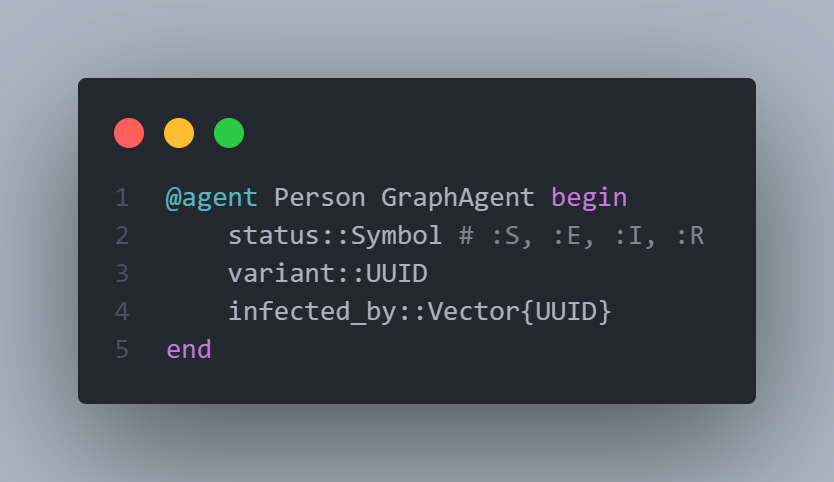
\includegraphics[width=\textwidth]{img/agent_code.png}
    \captionof{figure}{Codice Agente}
    \label{fig:Agent_code}
\end{minipage}

Come e' possibile vedere dalla Figura \ref{fig:Agent_code}, il codice che si occupa
di creare l'agente e' estremamente semplice. Al suo interno troviamo tutto quello che 
un agente deve sapere per poter agire in maniera corretta all'interno dell'ambiente. 
Essendo che l'agente \emph{Person} deriva dall'agente GraphAgent, questo eredita 
automaticamente i campi fondamentali \textbf{pos} e \textbf{id}, i quali serviranno 
per riconoscere la posizione all'interno del grafo dell'agente e distinguere l'agente 
dagli altri.

I campi principali sono:
\begin{itemize}
	\item status: e' un campo di tipo \textbf{Symbol} che rappresenta 
	lo stato di un determinato agente in un preciso momento del tempo. 
	Questo stato puo' mutare nel tempo ed e' strettamente correlato a 
	tutti e soli gli stati che un individuo puo' assumere all'interno di
	un modello matematico di tipologia \textbf{SEIR}
	\item variant:  e' un campo di tipo \textbf{UUID} (Universally Unique ID)
	che rappresenta un identificatore univoco associato ad una delle possibili
	varianti dell'agente patogeno attualmente in circolazione. Questo attributo 
	serve principalmente a gestire la possibilita' di non avere una completa
	immunita' dopo aver contratto e aver debellato il virus dal proprio sistema 
	immunitario, rendendo gli individui identificati come \textbf{:R} 
	passibili di reinfezione
	\item infected by: e' un campo di tipo \textbf{Vector} che rappresenta 
	quali varianti sono state contratte dall'agente. Un agente non puo' piu'
	essere infettato da queste varianti. Questo approccio e' stato ideato per 
	la modellazione di un vaccino, il quale non e' detto che copra tutte le
	varianti che sono uscite, o comunque non e' detto che, pur coprendo tutte le
	varianti conosciute copra anche quelle non conosciute.
\end{itemize}

Utilizzare la macro @agent e' il modo che viene incentivato dal linguaggio, in quanto
permette di creare un agente da un super tipo come AbstractAgent e permette di avere 
gia' inclusi tutti i campi necessari. Inoltre, utilizzando questa \textbf{macro} e' 
possibile includere tutti i campi di un altro agente, dovendo solamente specificare quelli 
nuovi.

\subsubsection*{Spazio e Modello}
Lo spazio e' di tipo GraphSpace e viene definito direttamente in 
fase di creazione del modello. 

\begin{minipage}{\linewidth}
    \centering
    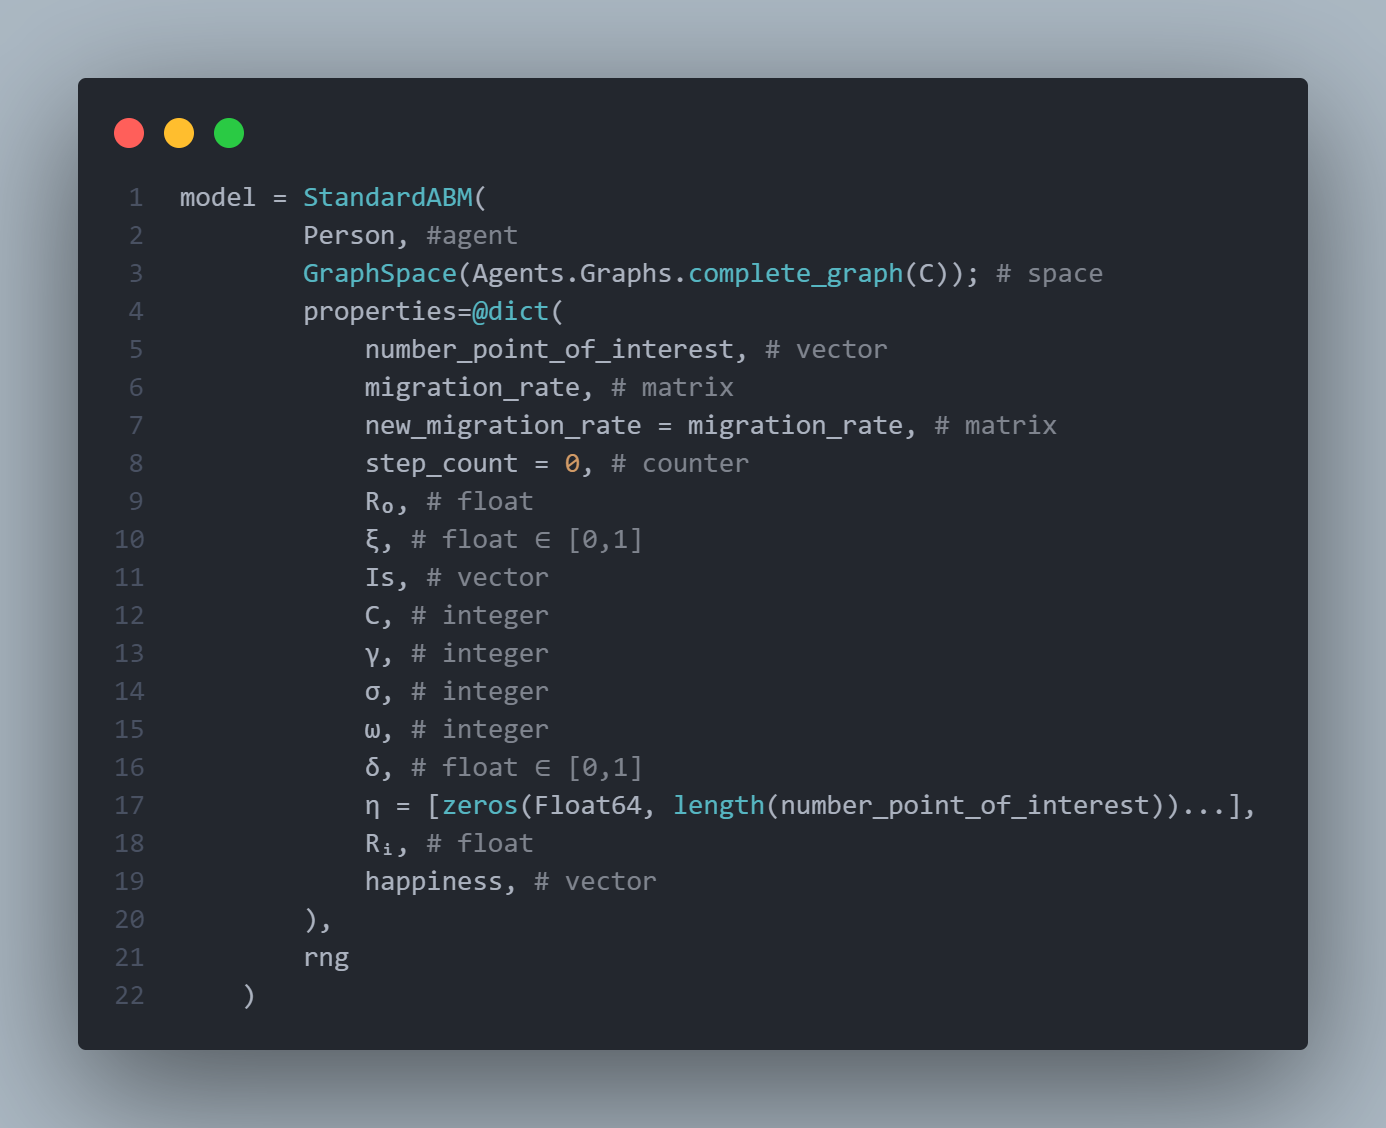
\includegraphics[width=\textwidth]{img/model_code.png}
    \captionof{figure}{Codice Modello}
    \label{fig:model_code}
\end{minipage}

In questo caso come si puo' osservare dalla Figura \ref{fig:model_code}, lo spazio 
e' un \emph{grafo completo} con C nodi. I nodi corrispondono ai punti di interesse del 
grafo. Per dettagliare maggiormente questo spazio altrimenti scarno, vengono definite delle 
\emph{proprieta' spaziali} del modello, ovvero proprieta' che ci sono sempre e ovunque. 
Queste proprieta' possono essere divise in due macro categorie: proprieta' dei punti di interesse
e proprieta' della pandemia.

Le proprieta' dei punti di interesse sono le seguenti:
\begin{itemize}
	\item number point of interest: e' di tipo \textbf{Vector} e rappresenta il numero di agenti 
	che quel determinato nodo puo' contenere.
	\item migration rate: e' di tipo \textbf{Matrix} e rappresenta una matrice di transizione tra i 
	vari nodi del grafo. Questa matrice di transizione codifica la probabilita' di un agente di spostarsi
	dal suo nodo ad un qualsiasi altro nodo presente. Essendo il grafo di tipo completo, ogni nodo 
	e' collegato a tutti gli altri, tuttavia non tutti i collegamenti sono equamente probabili.
	La matrice infatti tiene in considerazione la probabilita' di un agente di spostarsi piu' 
	facilmente verso un nodo popoloso, piuttosto che verso uno che non lo e', questo a mimica degli 
	spostamenti umani.
	\begin{minipage}{\linewidth}
		\centering
		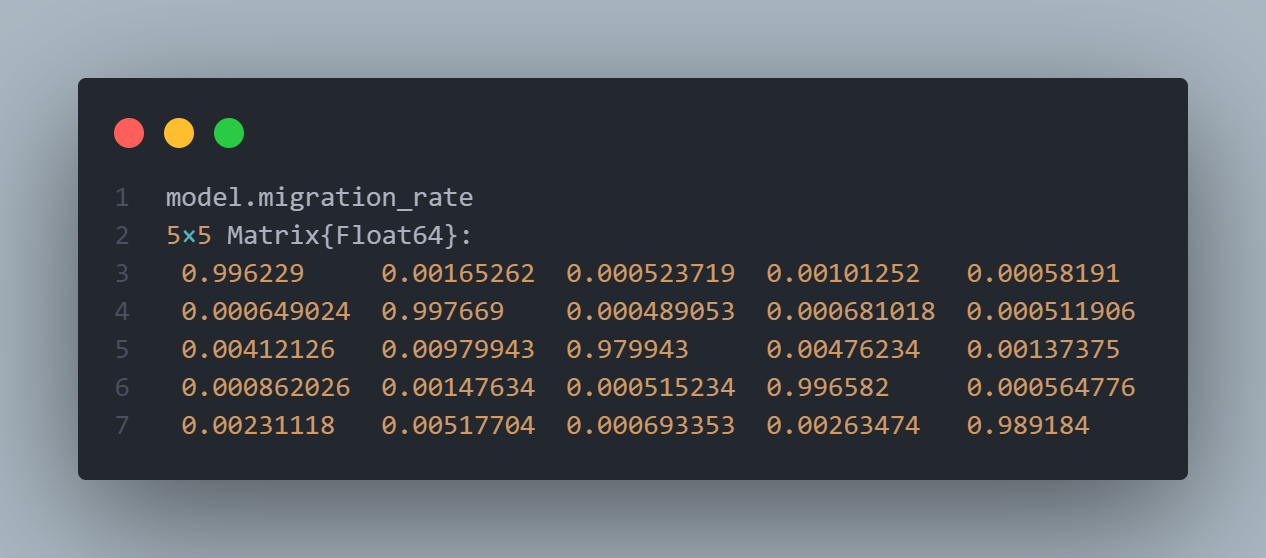
\includegraphics[width=\textwidth]{img/travel_rate.png}
		\captionof{figure}{Esempio di matrice di transizione}
		\label{fig:migration_matrix}
	\end{minipage}
	\item Is: e' di tipo \textbf{Vector} e rappresenta il vettore degli infetti iniziali.
	Generalmente viene inizializzato randomicamente nella posizione dei nodi, ma fisso nel numero
	di infetti ovvero con I = 1. 
	\item $\eta$: e' di tipo \textbf{Vector} e rappresenta il vettore delle contromisure implementate.
	L'esperienza della pandemia ci ha insegnato che non sempre una contromisura generalizzata e' qualcosa
	che funziona, alle volte e' giusto trattare in maniera locale il problema, applicando contromisure mirate
	alla tipologia di esigenza locale. Questo vettore raccoglie quindi le contromisure associate ad ogni 
	nodo del grafo. Una contromisura e' un valore $\in [0,1]$ che identifica l'efficacia della contromisure applicate.
	La sfida e' comprendere in che modo una contromisura impatti sulla diffusione della pandemia.
	\item happiness: e' di tipo \textbf{Vector} e rappresenta il vettore della felicita' della popolazione 
	di un determinato nodo. Questo vettore contiene valori $\in [-1,1]$. Questo parametro e' stato inserito 
	per evitare una caduta in una strategia funzionale ma insostenibile. Se l'obiettivo di un controllore 
	e' quello di minimizzare il numero di infetti (e morti), la scelta piu' ragionevole (non dovendo tenere 
	in conto di null'altro), e' quella di applicare un lockdown generalizzato a tutta la popolazione. 
	Terminato il periodo di vita del virus si e' risolta la crisi pandemica. Questa soluzione e' pero'
	\textbf{umanamente insostenibile}. Da qui un termine aggiuntivo che il controllore deve bilanciare, 
	ovvero la felicita' della popolazione. Infatti questo termine deve essere massimizzato, e dipende 
	principalmente dal termine $\eta$.
\end{itemize}

Le proprieta' della pandemia sono invece:
\begin{itemize}
	\item $R_0$: e' di tipo \textbf{Float64} e rappresenta l'indice di infettivita' di un virus
	\item $\gamma$: e' di tipo \textbf{Int} e rappresenta il numero di giorni dopo di cui un paziente
	che ha contratto il virus puo' considerarsi guarito
	\item $\sigma$: e' di tipo \textbf{Int} e rappresenta il numero di giorni per cui un agente dopo essere
	stato infettato viene considerato \emph{esposto}, per cui non ancora in grado di infettare, ma che una 
	volta terminato questo periodo diventera' infettivo
	\item $\omega$: e' di tipo \textbf{Int} e rappresenta il numero di giorni per cui un agente e' considerato
	immune alla malattia dopo essere guarito da essa
	\item $\delta$: e' di tipo \textbf{Float64} e rappresenta la probabilita' di un agente infetto di morire al 
	termine del proprio periodo di infettivita' ($\gamma$).
	\item $\xi$: e' di tipo \textbf{Float64} $\in [0,1]$ e rappresenta, una volta che e' stato introdotto un vaccino come metodo 
	di prevenzione controil virus, il rateo di individui S che che possono essere vaccinati, e quindi diventare R,
	al giorno.
	\item $R_i$: e' di tipo \textbf{Float64} e rappresenta l'indice di infettivita' desiderato, che si vuole
	raggiungere per arginare la malattia e fermarne l'avanzata. Generalmente questo valore si attesta al piu' 
	intorno a 1.0
\end{itemize}

\subsubsection*{Scelta parametri}

\subsubsection*{Funzione di avanzamento agente}

\subsubsection*{Funzione di avanzamento modello}

\subsubsection*{Grafici}

Descrizione approfondita del modello ad agente usato.
Spiegazione della tipologia di spazio, del perche' e' usato, e 
dell'agente. 

Spiegazione dei parametri utilizzati e del perche' sono stati 
scelti in quel modo. Spiegazione di come vado a ottenere tali parametri 
e i dati su cui faccio affidamento.

Risultati grafici.